% vim: set textwidth=78 autoindent:
% !TeX root = user_guide.tex

\section{MapServer Export Plugin}\label{sec:mapserver_export}
\index{Plugins!MapServer Export}

% when the revision of a chapter has been finalized, 
% comment out the following line:
% \updatedisclaimer

Mit dem Plugin \toolbtntwo{mapserver_export}{MapServer Export} k�nnen Sie
eine Map-Datei f�r den UMN MapServer erstellen. Dazu verwenden Sie QGIS, um
die Layer im Kartenfenster zu arrangieren, zu beschriften und die Farben nach
ihren W�nschen anzupassen und speichern das Ergebnis als QGIS Projekt ab.

\subsection{Eine Projektdatei f�r das MapServer Export Plugin erstellen}

Das MapServer Export Plugin verwendet eine gespeicherte QGIS Projektdatei und
nicht die aktuell im Kartenfenster angezeigten Layer. Dies hat bereits
h�ufiger zu Verwirrung gef�hrt. Wie im weiteren Verlauf beschrieben, m�ssen
Sie die Layer im Kartenfenster layouten und dann als Projekt abspeichern.

\begin{figure}[ht]
\begin{center}
  \caption{Layer im Kartenfenster layouten und als Projekt speichern \nixcaption}
  \label{fig:mapserver_export_qgs}\smallskip
  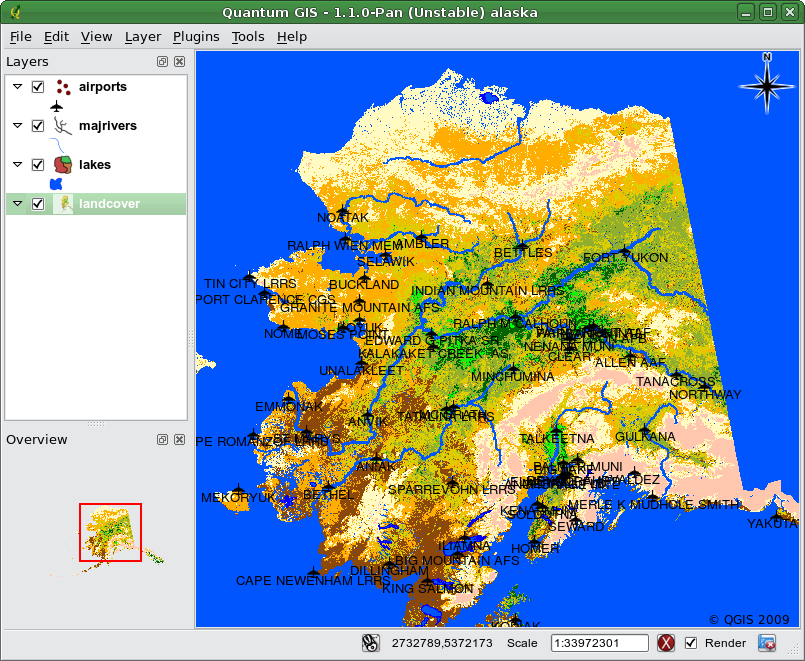
\includegraphics[clip=true, width=12cm]{mapserver_export_qgis}
\end{center}
\end{figure}

In diesem Beispiel wird in vier Schritten gezeigt, wie Sie zu dem Punkt
kommen, an dem Sie die Map-Datei erstellen k�nnen. Wir verwenden dazu Raster-
und Vektorlayer aus dem QGIS Beispieldatensatz \ref{label_sampledata}.

\begin{enumerate}
\item Laden Sie den Rasterlayer \filename{landcover.img}, indem Sie auf das
Icon \toolbtntwo{mActionAddRasterLayer}{Add Raster Layer} klicken.
\item F�gen Sie den Vektorlayer \filename{lakes.gml, majrivers.shp} und 
\filename{airports} aus dem QGIS Beispieldatensatz hinzu, indem Sie das Icon
\toolbtntwo{mActionAddNonDbLayer}{Add Vector Layer} verwenden.
\item �ndern Sie die Farben und Beschriftung nach ihren W�nschen (siehe
Abbildung~\ref{fig:mapserver_export_qgs})
\item Speichern Sie das neue Projekt unter dem Namen
\filename{mapserverproject.qgs} im Men� \mainmenuopt{Datei} \arrow
\dropmenuopttwo{mActionFileSaveAs}{Projekt speichern als}.
\end{enumerate} 

\subsection{Eine Map-Datei erstellen}


Das Programm \filename{msexport} befindet sich im QGIS Programmordner und kann
unabh�ngig von QGIS verwendet werden. Von QGIS aus m�ssen Sie das MapServer
Export Plugin erst mit dem Plugin Manager laden. Klicken Sie dazu auf
\mainmenuopt{Plugins} \arrow \dropmenuopt{Plugins verwalten}, w�hlen Sie das
Plugin aus und klicken dann auf \button{OK}

Nun k�nnen Sie auf das Icon \toolbtntwo{mapserver_export}{MapServer Export}
in der Werkzeugleiste klicken und den Dialog \dialog{Exportieren in
MapServer} �ffnen (siehe Abbildung~\ref{fig:mapserver_export_dialog}). 

\begin{figure}[ht]
\begin{center}
  \caption{Dialog MapServer Export \nixcaption}
  \label{fig:mapserver_export_dialog}\smallskip
  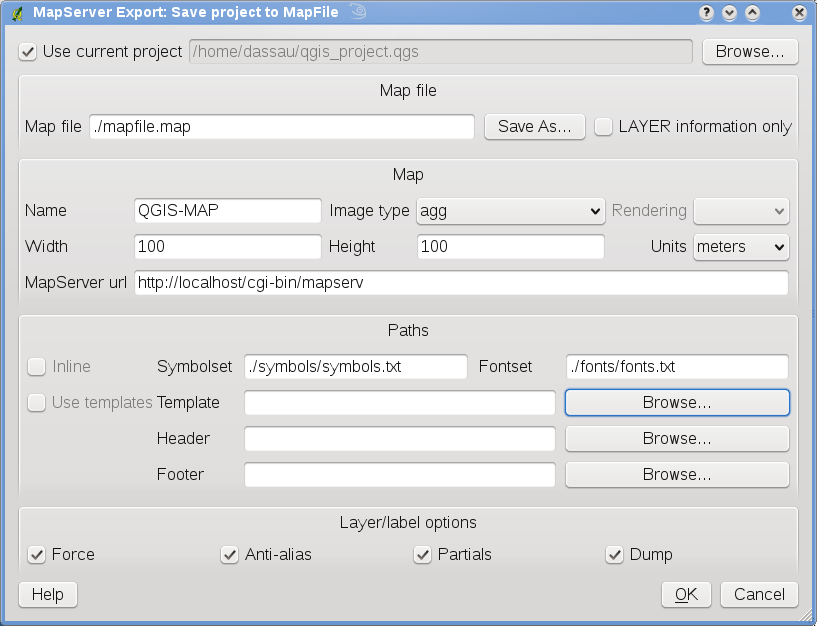
\includegraphics[clip=true, width=10cm]{mapserver_export_dialog}
\end{center}
\end{figure}

Hier ist eine Zusammenfassung der Eingabefelder:

\begin{description}
\item [Kartendatei] \mbox{}\\
Tragen Sie hier den Namen der Map-Datei ein, die erstellt werden soll. Sie
k�nnen mit dem 'Speichern unter' Knopf ausw�hlen, wo die Datei gespeichert
werden soll.
\item [QGIS Projektdatei] \mbox{}\\
Geben Sie den kompletten Pfad zur QGIS Projektdatei (.qgs) an, die Sie
exportieren m�chten. Sie k�nnen mit dem 'Durchsuchen' Knopf nach der
Projektdatei suchen.
\item [Name] \mbox{}\\
Ein Name f�r die Karte. Dieser Name wird als Prefix f�r alle durch den
MapServer erstellten Karten verwendet.
\item [Breite] \mbox{}\\
Breite des Ausgabebildes in Pixeln.
\item [H�he] \mbox{}\\
H�he des Ausgabebildes in Pixeln.
\item [Einheiten] \mbox{}\\
Ma�einheiten f�r die Ausgabe
\item [Bildtyp] \mbox{}\\
Bildformat, das vom MapServer erstellt wird
\item [Vorlage] \mbox{}\\
Kompletter Pfad zur MapServer Template-Datei, die mit der Map-Datei benutzt
wird
\item [Kopfzeile] \mbox{}\\
Kompletter Pfad zur MapServer Header-Datei, die mit der Map-Datei benutzt
wird
\item [Fusszeile] \mbox{}\\
Kompletter Pfad zur MapServer Footer-Datei, die mit der Map-Datei benutzt
wird
\end{description}

Nur die QGIS Projektdatei ist nun notwendig, um eine Map-Datei zu erstellen.
Es kann aber sein, dass diese nicht auf anhieb funktioniert, abh�ngig davon,
was sie sich vorstellen. Auch wenn QGIS durchaus geeignet ist, eine Map-Datei zu
erstellen, ist es h�ufig doch notwendig, die Map-Datei manuell
nachzubearbeiten. man sollte es daher eher als eine Hilfe betrachten, um die
Map-Datei nicht komplett neu erstellen zu m�ssen.

Aber lassen Sie uns in einem Beispiel anschauen, wie man aus der gerade
erstellten Projektdatei eine Map-Datei erstellt (siehe
Abbildung~\ref{fig:mapserver_export_dialog}).

\begin{enumerate}
  \item Klicken Sie auf das Icon \toolbtntwo{mapserver_export}{MapServer Export}.
  \item Geben Sie als Kartendatei \filename{qgisproject.map} f�r die neue
Map-Datei an.
  \item Geben Sie als QGIS Projektdatei die gerade erstellte Datei
\filename{mapserverproject.qgs} an.
  \item Geben Sie den Namen \filename{MyMap} f�r die Karte an.
  \item Geben Sie als Breite \filename{600} und als H�he \filename{400} an.
  \item Die Layer sind in feet, also �ndern wir die Einheit in Fu�.
  \item W�hlen Sie ``png'' als Bildtyp.
  \item Klicken Sie auf \button{OK}, um die neue Map-Datei
\filename{qgisproject.map} zu erstellen. QGIS zeigt an, dass es erfolgreich
war.
\end{enumerate}

Sie k�nnen sich die Map-Datei in einem Texteditor anschauen. Sie werden
sehen, dass das Exportmodul alle Metadaten hinzugef�gt hat, um die Map-Datei
f�r WMS zu aktivieren.

\subsection{Testen der Map-Datei}

Sie k�nnen die Map-Datei testen, indem Sie ein Bild mit dem Programm
\filename{shp2img} erzeugen (siehe
Abbildung~\ref{fig:mapserver_export_test}). \filename{shp2img} ist Teil der
UMN MapServer Installation, aber es ist auch in dem Programm FWTools
vorhanden. Um ein Testbild zu erstellen sind folgende Schritte notwendig:

\begin{figure}[ht]
\begin{center}
  \caption{Testbild erstellt mit dem Programm shp2img \nixcaption}
  \label{fig:mapserver_export_test}\smallskip
  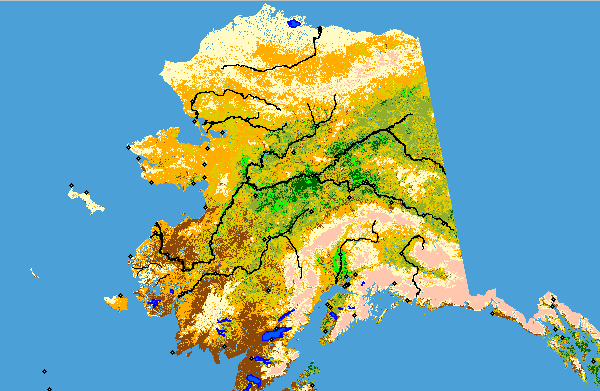
\includegraphics[clip=true, width=12cm]{mapserver_export_test}
\end{center}
\end{figure}

\begin{itemize}[label=--]
\item �ffnen wir eine Shell, damit wir das Programm shp2img aus der
Kommandozeile starten k�nnen.
\item Wenn die Map-Datei nicht im aktuellen Verzeichnis gespeichert wurde,
wechseln Sie bitte in das entsprechende Verzeichnis mit der Map-Datei
\item starten Sie \filename{shp2img -m qgisproject.map -o mapserver\_test.png}
\item Schauen Sie sich das erstellte Bild mit einem Bildbetrachter an
\end{itemize}

Die Ausdehnung des Bildes ist exakt diejenige, die wir in der QGIS-Projektdatei
abgespeichert haben. Und das erstellte PNG enth�lt alle Layer, die wir als
QGIS-Projekt abgespeichert haben, au�er den airport Symbolen.

Wenn Sie vorhaben, die Map-Datei auch f�r WMS-Anfragen zu nutzen, dann
brauchen Sie wahrscheinlich nichts weiter zu machen. Wenn Sie es als
Kartenvorlage oder individuelle Oberfl�che nutzen wollen, ist wahrscheinlich
noch ein bischen manuelles Optimieren notwendig. Um zu sehen, wie einfach es
ist, Karten aus QGIS ins Internet zu stellen, schauen Sie sich das 5-min�tige
Flashvideo von Christopher Schmidt an, auch wenn es auf einer �lteren QGIS
Version basiert:
\footnote{\url{http://openlayers.org/presentations/mappingyourdata/}}

\FloatBarrier

